\chapter{Selective Saturation and Brightness for Visualizing Time-Varying Volume Data}
Time-varying volume data is used in many areas of science and engineering. However visualizations of such data are not easy for users to visually process due to the amount of information that can be presented simultaneously. In this chapter, we propose a novel visualization approach which modulates focus, emphasizing important information, by adjusting saturation and brightness of voxels based on an importance measure derived from temporal and multivariate information. By conducting a voxel-wise analysis of a number of consecutive frames, we acquire a volatility measure of each voxel. We then use intensity, volatility and additional multivariate information to determine opacity, saturation and brightness of the voxels. The method was tested in visualizing a multivariate hurricane data set. The results suggest that our approach can give the user a more detailed understanding of the data by presenting multivariate information variables in one self-contained visualization.

%-------------------------------------------------------------------------
\section{Introduction}
With the development of more advanced techniques for scientific simulation, where various physical measurements at many time-steps can be simulated at extremely high detail, providing intuitive and effective tools for the analysis and visualization of such data becomes increasingly challenging.

Color mappings are often used in visualization to represent various types of information. Although traditional color transfer functions are often in RGB color space, transfer functions designed in HSB (hue, saturation and brightness) color space can be more intuitive and meaningful in terms of conveying quantitative information or for classifications of the data.
%-------------------------------------------------------------------------
\section{Related Work}
The visualization of time-varying data is an important and active topic in the visualization community. Transfer function specification for static volume data has been widely studied over the years \cite{pfister_transfer_2001}. However, less work has been done for transfer function design of time-varying data.

Jankun-Kelly and Ma first studied  transfer function specification for time-varying data \cite{jankun-kelly_study_2001}.
Kniss and Hansen applied the techniques from multi-dimensional transfer function based volume rendering to the visualization of multivariate data from weather simulations \cite{kniss_volume_2002}.
%Akiba et al. presented the use of time histogram for simultaneous classification of time-varying data in order to find transfer functions that classify all the time steps of the data set \cite{akiba_simultaneous_2006}.
%Woodring and Shen presented a method for the comparison of different data fields through the expression of a volume shader that composes data fields together with set operations \cite{woodring_multi-variate_2006}.
%Wang et al. introduced an importance measure based on conditional entropy and categorize temporal behaviors by clustering the importance curves over time \cite{wang_importance-driven_2008}.

%Data analysis techniques for high dimensional spaces, such as parallel coordinates \cite{akiba_visualizing_2007} \cite{guo_scalable_2012} and principal component analysis \cite{liu_multivariate_2014}, were also investigated for exploring multivariate time-varying data sets.

%\cite{luo_information-guided_2014}.

Akiba et al. \cite{akiba_visualizing_2007} described three approaches for the data-fusion problem in multivariate data visualization.
One approach, which is to use one variable for each color channel in RGB space, is popular because of its simplicity but is limiting due to the difficulty for viewers to interpret the resulting color.
The second approach, is to use one of the values based on some criterion e.g. \cite{hastreiter_integrated_1998}
use alternating sampling for rendering two volumes and this has been shown to work well for medical imaging but not for fluid flow visualization.
The third approach is to compute a weighted sum of all the values. This approach is more flexible however this may not be guaranteed to lead to an effective visualization as blending different colors might lead to ambiguous mixing of different hues.

%for the last point: SHOULD EXPLAIN WHY?


%-------------------------------------------------------------------------
\section{Method}
In this poster, we propose an intuitive approach of using color mappings in HSB space to effectively represent multivariate time-variant data. We use opacity to represent the main variable and saturation to represent the volatility of the main variable. In addition brightness can be used to represent other information such as an additional variable from a multivariate or multi-dimensional data set. 

%Figure~\ref{fig:saturation_brightness} is a 2D map where saturation is mapped to the x axis and brightness to the y axis. It illustrates how the look of red color and cyan color change when their saturation and brightness vary.

For a multivariate data set with two variables X, Y, we use variable X of voxels for the alpha channel and modulate the saliency of voxels by adjusting saturation and brightness based on the volatility of variable X and the values of variable Y respectively.
The volatility is measured by temporal standard deviation std(i), which is the standard deviation of the i-th voxel in the recent n consecutive frames, where n is a user specified number.
%We use temporal standard deviation of voxels as a measure of volatility. The temporal standard deviation std(i) is acquired by calculating standard deviation of the i-th voxel in the recent n consecutive frames, where n is a user specified number.
The hue, saturation, brightness and alpha of the i-th voxel (an element in a volume data set) in HSB color space are defined as follows:
\begin{align*}
Hue(i) = C(i) \\
Saturation(i) = Clip(a \times std(i)) \\
Brightness(i) = 1-Clip(b \times Y(i)) \\
Alpha(i) = X(i) 
\end{align*}
where std(i) is the volatility and C(i) can be either a user-specified constant hue or mapped to a variable such as X(i). Clip is a function that clips the value to the range [0, 1]. $a$ and $b$ are scale factors for saturation and brightness respectively, which are determined by the user based on the distribution of variables X and Y in the data set. Variables X(i) and Y(i) are normalized to the range [0, 1].

%\begin{figure}
%\centering
%\begin{minipage}{.15\textwidth}
%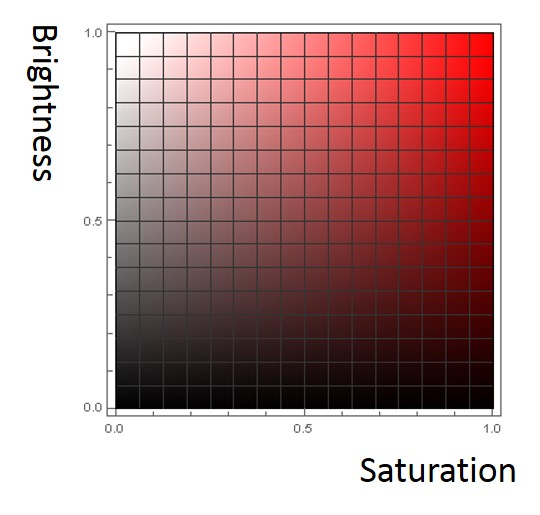
\includegraphics[width=1\linewidth]{images/saturation_brightness_red.jpg}
%\end{minipage}~
%\begin{minipage}{.15\textwidth}
%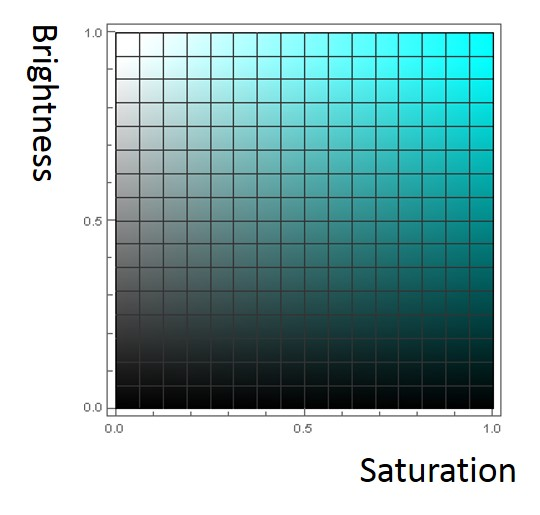
\includegraphics[width=1\linewidth]{images/saturation_brightness_cyan.jpg}
%\end{minipage}~
%\caption{Various saturation and brightness of red and cyan}
%\label{fig:saturation_brightness}
%\end{figure}


%\begin{figure}
%\centering
%\begin{minipage}{.15\textwidth}
%\centering
%\includegraphics[width=1\linewidth]{images/article-color-value-saturation-200x53}
%\caption{Varying saturation from 1 to 0}
%\label{fig:color-value-saturation}
%\end{minipage}~
%\begin{minipage}{.15\textwidth}
%\centering
%\includegraphics[width=1\linewidth]{images/article-color-value-brightness-200x52}
%\caption{Varying brightness from 1 to 0}
%\label{fig:color-value-brightness}
%\end{minipage}~
%\begin{minipage}{.15\textwidth}
%\centering
%\includegraphics[width=1\linewidth]{images/article-color-value-brightness-saturation-200x49}
%\caption{Saturation and brightness from (1, 1) to (0, 0.5)}
%\label{fig:color-value-brightness-saturation}
%\end{minipage}
%\end{figure}

% Task driven color coding \cite{tominski_task-driven_2008}
% Color scheme \cite{harrower_colorbrewer.org:_2003}

%-------------------------------------------------------------------------
\section{Results}
We tested our method on the hurricane data set from the National Center for Atmospheric Research provided for the IEEE Visualization 2004 Contest.
The hurricane model is Hurricane Isabel, which was a very strong hurricane in the west Atlantic region in September of 2003.
%The size of the data set is 500 (longitude) $ \times $ 500 (latitude) $ \times $ 100 (height) $ \times $ 48 (time). One time-step is one hour in the simulation.
The variables we used in the tests are cloud moisture mixing ratio (kg water/kg dry air) and total precipitation mixing ratio (sum of mixing ratios of graupel, rain and snow). The ground in the hurricane data set, which is a height field of the surface topography, is rendered with relief mapping and presented as background in the visualization results.

In Figure~\ref{fig:hurricane_gray}, the cloud, volatility of cloud and precipitation at frame 40 are displayed in grayscale for comparison.
Figure~\ref{fig:hurricane_frames} shows images of 3 frames of the hurricane rendered with cloud, volatility of cloud and precipitation. Cloud is used as variable X and precipitation as variable Y. The temporal standard deviation is calculated using the recent 10 frames.
The strong red color near the hurricane eye indicates where the hurricane was in previous several frames and the clouds with more precipitation are darker in the images.
%Figure~\ref{fig:hurricane_40_cyan} displays a more realistic rendering of the same frame in Figure~\ref{fig:hurricane_40_defaultangle}, with a cyan hue and used precipitation to adjust both saturation and brightness.

\begin{figure}
\centering
\begin{minipage}{.15\textwidth}
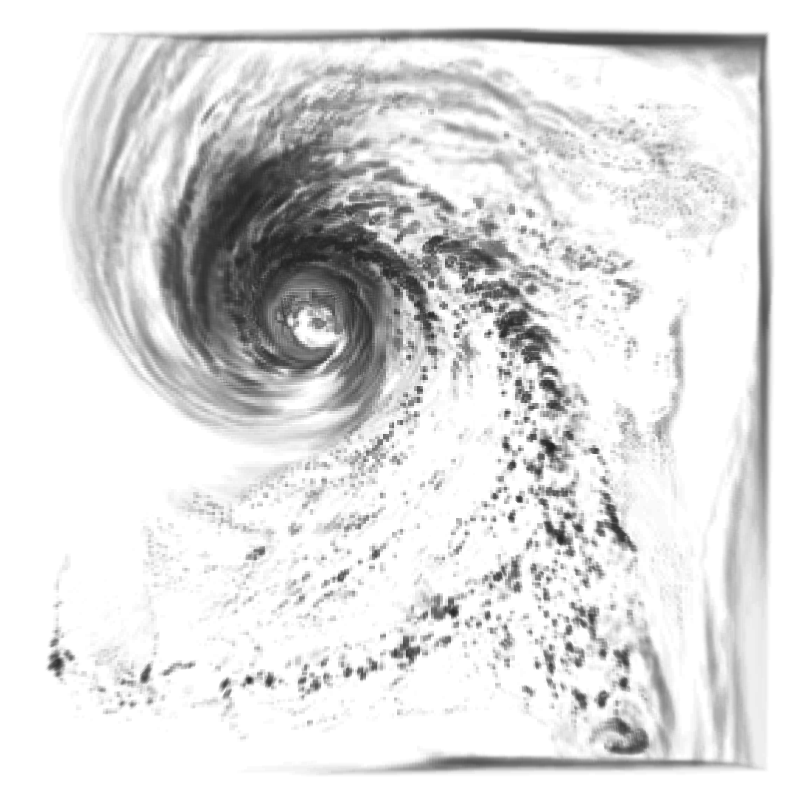
\includegraphics[width=1\linewidth]{images/hurricane_cloud_gray_40}
%\caption{Cloud at frame 40}
%\label{fig:hurricane_cloud_gray}
\end{minipage}~
\begin{minipage}{.15\textwidth}
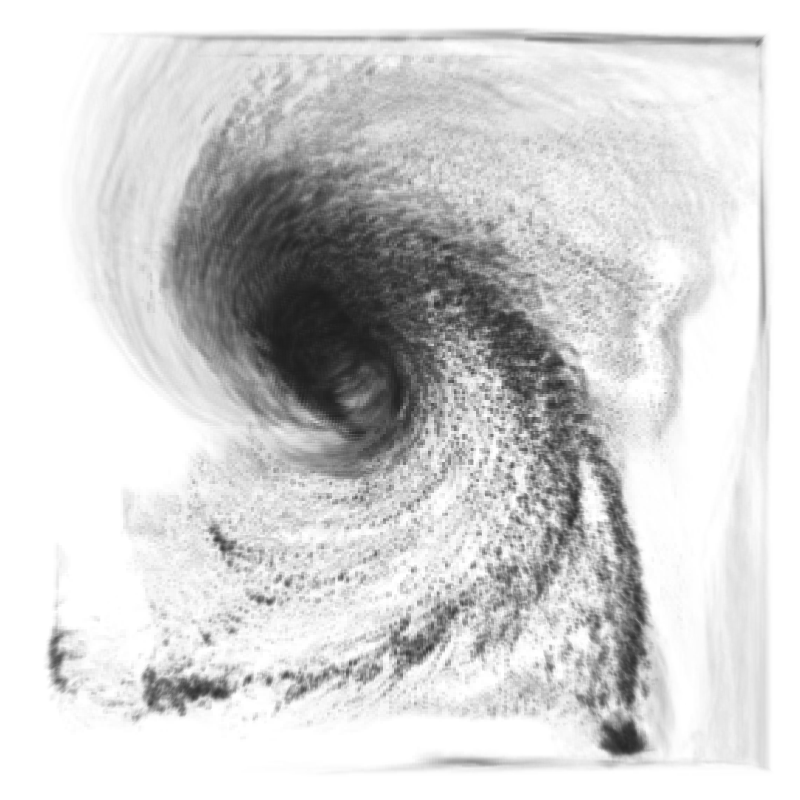
\includegraphics[width=1\linewidth]{images/hurricane_std_gray_40}
%\caption{Volatility of cloud at frame 40}
%\label{fig:hurricane_std_gray}
\end{minipage}~
\begin{minipage}{.15\textwidth}
\centering
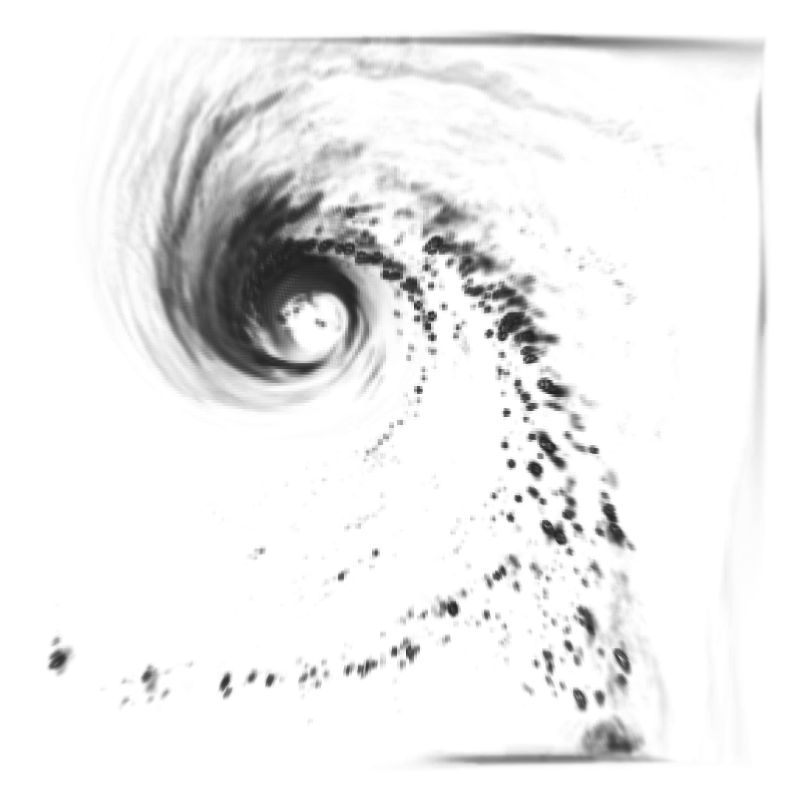
\includegraphics[width=1\linewidth]{images/hurricane_precip_gray_40}
%\caption{Precipitation at frame 40}
%\label{fig:hurricane_precip_gray}
\end{minipage}
\caption{Cloud (left), volatility of cloud (middle) and precipitation (right) at frame 40}
\label{fig:hurricane_gray}
\end{figure}

\begin{figure}
\centering
\begin{minipage}{.15\textwidth}
\centering
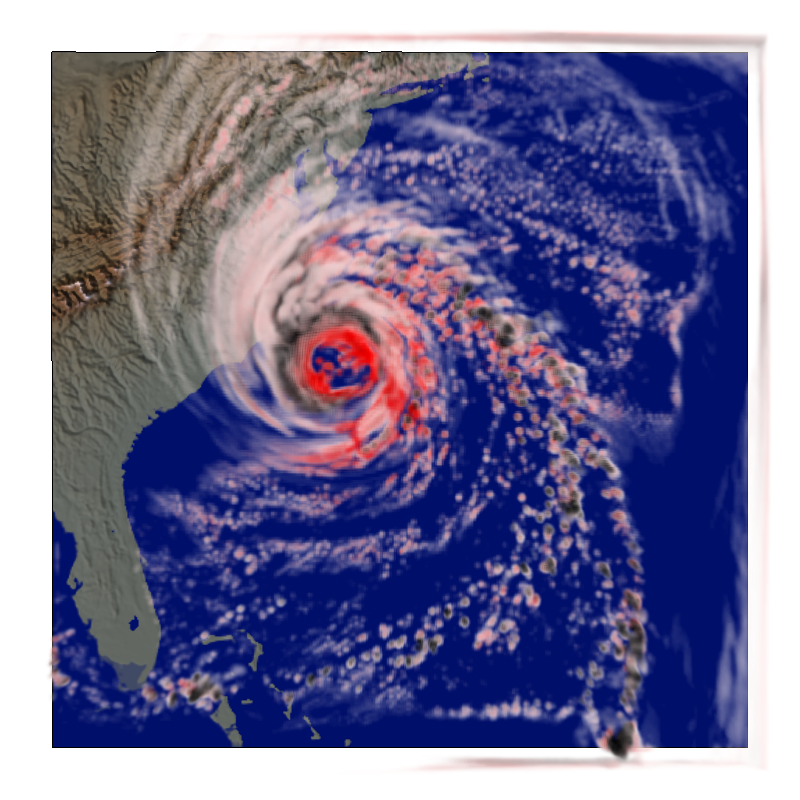
\includegraphics[width=1\linewidth]{images/hsba_0_10std_1-10precip_cloud_35}
\end{minipage}~
\begin{minipage}{.15\textwidth}
\centering
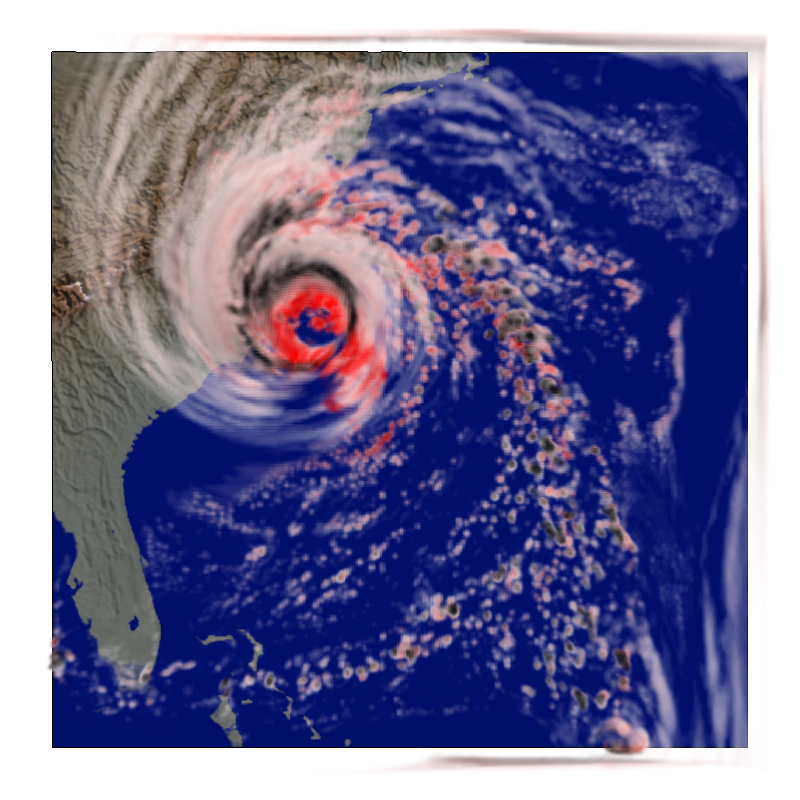
\includegraphics[width=1\linewidth]{images/hsba_0_10std_1-10precip_cloud_40}
\end{minipage}~
\begin{minipage}{.15\textwidth}
\centering
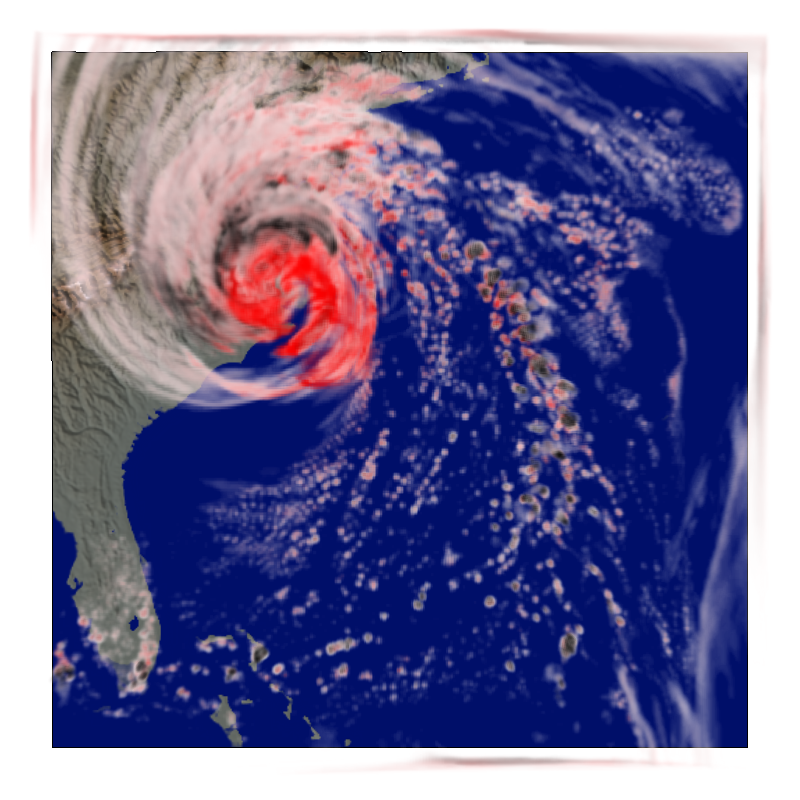
\includegraphics[width=1\linewidth]{images/hsba_0_10std_1-10precip_cloud_45}
\end{minipage}
\caption{Adjusting saturation and brightness of frame 35 (left), frame 40 (middle) and frame 45 (right)}
\label{fig:hurricane_frames}
\end{figure}

%We also tested our method on a time-varying smoke simulation based on an implementation of \cite{fedkiw_visual_2001}. Figure~\ref{fig:smoke} to Figure~\ref{fig:smoke_gradient} are smoke density, volatility of smoke density and gradient magnitude of smoke density rendered in grayscale for comparison.
%The gradient magnitude is the Euclidean norm of the gradient at a voxel position,
%% approximated using discrete derivatives of Gaussians in each dimension.
%and the temporal standard deviation is calculated using the recent 10 frames.
%In Figure~\ref{fig:smoke_hsba_red}, smoke density is used as variable X and gradient magnitude as variable Y. The image was rendered with a constant hue (red) and parameters $a=10$ and $b=5$ were used. 
%
%\begin{figure}
%\centering
%%\begin{minipage}{.24\textwidth}
%%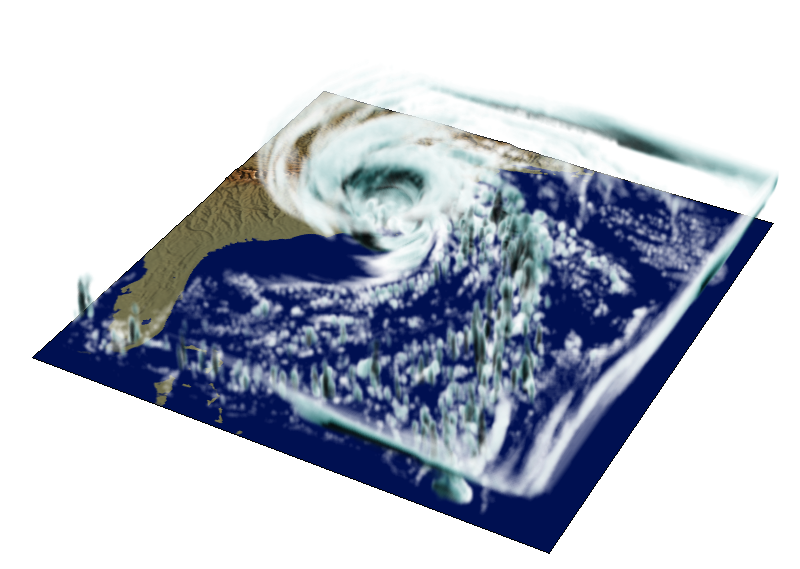
\includegraphics[width=1\linewidth]{images/hsba_cyan_10precip_1-10precip_cloud_40_defaultangle}
%%\caption{A more realistic rendering with both saturation and brightness representing precipitation at frame 40. Hue is cyan, a=10 and b=10}
%%\label{fig:hurricane_40_cyan}
%%\end{minipage}
%
%\begin{minipage}{.10\textwidth}
%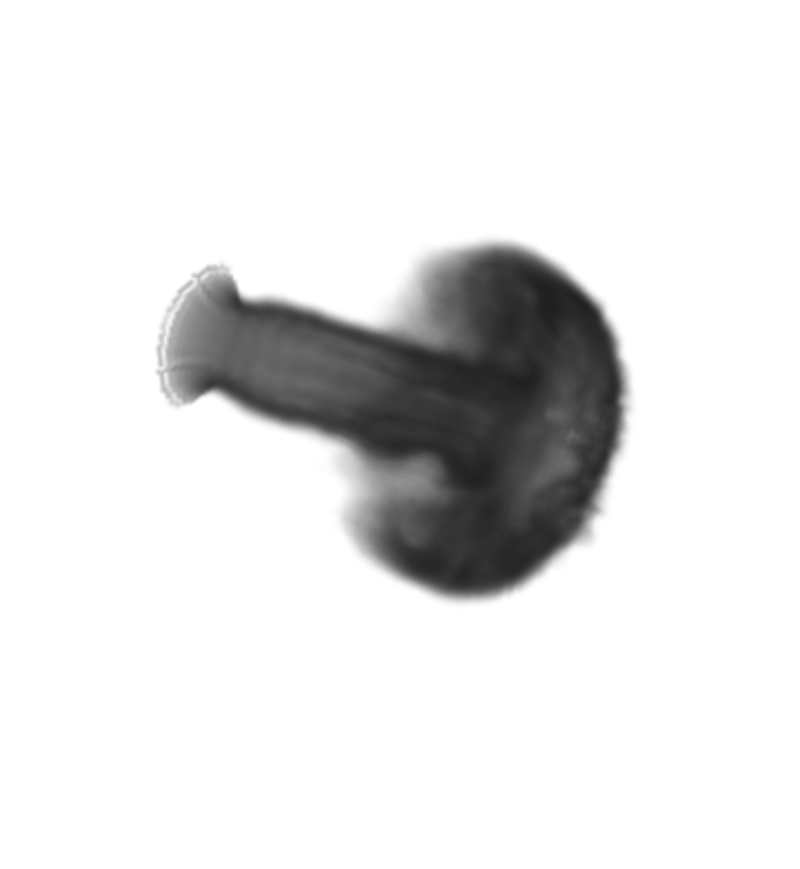
\includegraphics[width=1\linewidth]{images/smoke_160_.png}
%\caption{Smoke density at frame 160}
%\label{fig:smoke}
%\end{minipage}~
%\begin{minipage}{.10\textwidth}
%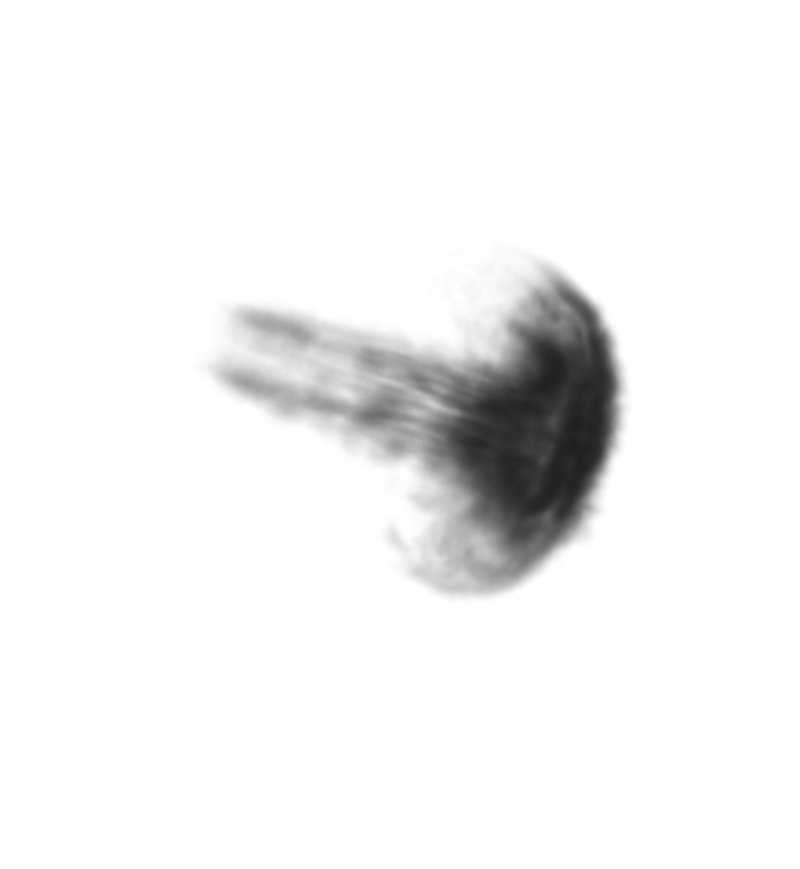
\includegraphics[width=1\linewidth]{images/smoke_std_160_.png}
%\caption{Smoke volatility at frame 160}
%\label{fig:smoke_std}
%\end{minipage}~
%\begin{minipage}{.10\textwidth}
%\centering
%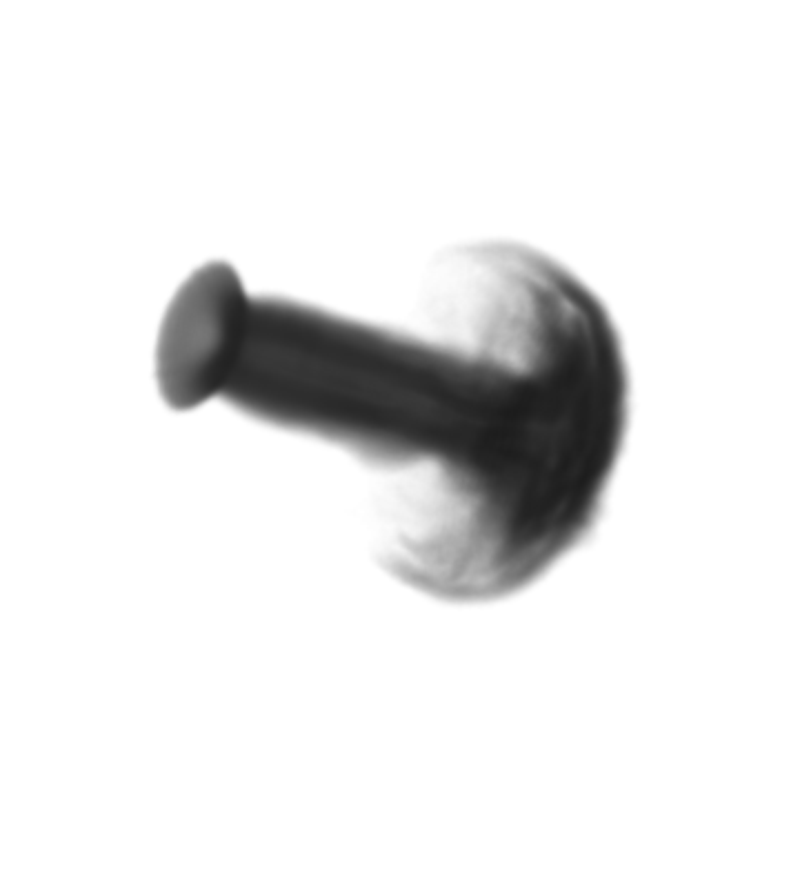
\includegraphics[width=1\linewidth]{images/smoke_gradient_160_.png}
%\caption{Smoke gradient magnitude at frame 160}
%\label{fig:smoke_gradient}
%\end{minipage}~
%%\begin{minipage}{.24\textwidth}
%%	\centering
%%	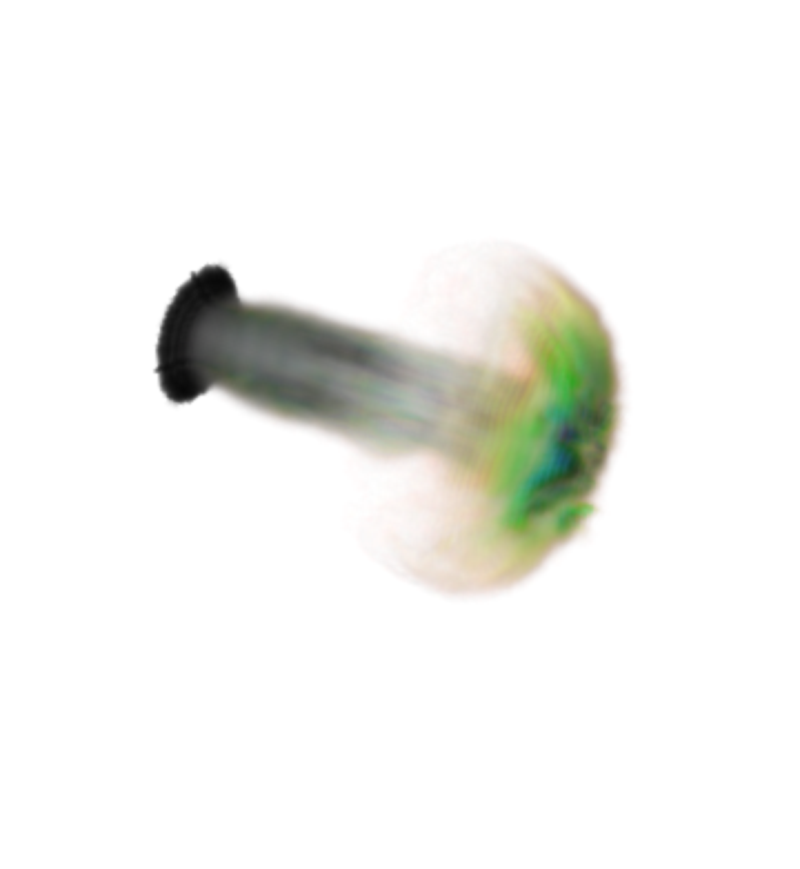
\includegraphics[width=1\linewidth]{images/smoke_hsba_intensity_10std_5gradient_intensity_160.png}
%%	\caption{Smoke density as variable X and gradient magnitude as variable Y at frame 160. Hue is X(i), a=10 and b=5}
%%	\label{fig:smoke_hsba_intensity}
%%\end{minipage}~
%\begin{minipage}{.15\textwidth}
%	\centering
%	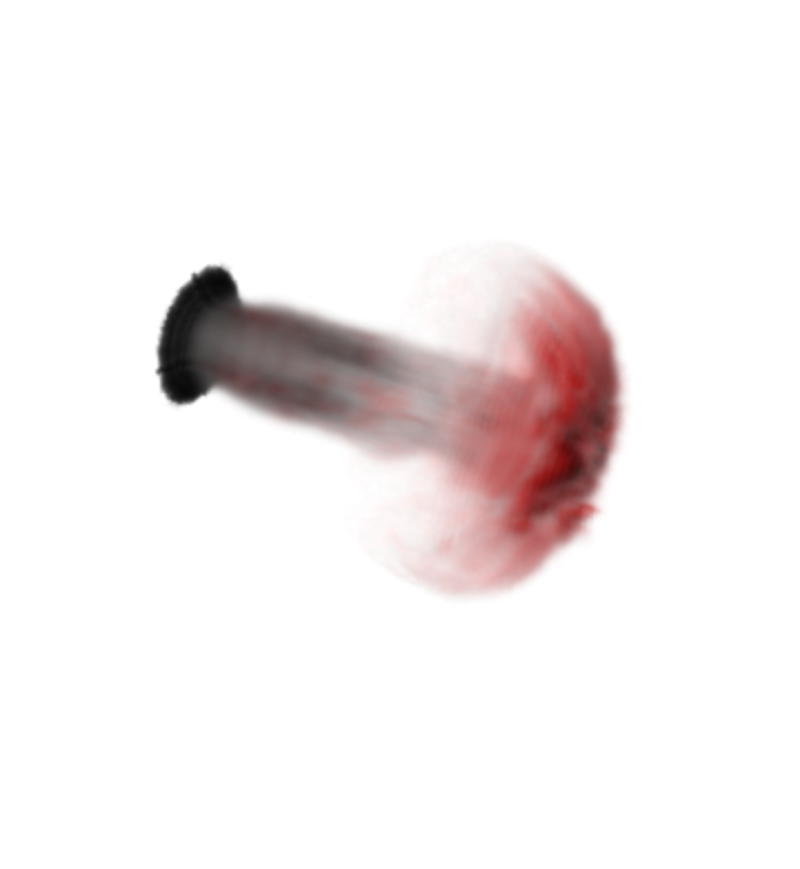
\includegraphics[width=1\linewidth]{images/smoke_hsba_red_10std_5gradient_intensity_160.png}
%	\caption{Part of the smoke is desaturated and darkened.}
%	\label{fig:smoke_hsba_red}
%\end{minipage}
%\end{figure}

%-------------------------------------------------------------------------
\section{Conclusions}
Our main contribution is a mechanism for exploiting saturation and brightness to modulate focus in time-variant volume visualization using an importance measure that is based on volatility. In addition we demonstrate how additional variables in a multivariate data set could be communicated simultaneously through the brightness channel. Preliminary results indicate that the results can provide more visual information for the test data set. In future work we plan to conduct perceptual experiments to quantitatively evaluate the mechanism and determine the optimal parameters for the approach.

%-------------------------------------------------------------------------
